\section{Compactness and sequential compactness}
\label{compactness}
\subsection{Compactness}
\begin{defn}
  Let $(X,\calT)$ be a topological space.
  \begin{enumerate}
    \item[(i)] A collection $\calU \subset \calT$ of open sets of called an \wordexp{open~cover}{{\"o}ppen~{\"o}vert{\"a}ckning}{cover}{{\"o}vert{\"a}ckning} of $X$ if $X = \bigcup_{U \in \calU} U$.
    \item[(ii)] The space $X$ is called \word{compact}{kompakt} if \emph{every} open cover $\calU$ of $X$ has a finite subcover, meaning that one can find finitely many open sets $U_1, \dots, U_n \in \calU$ so that $X = \bigcup_{i=1}^n U_i$.
  \end{enumerate}
\end{defn}
\trans{cover}{{\"o}vert{\"a}ckning}
\trans{compact}{kompakt}
\begin{example}
  Every finite topological space is compact, since there are only finitely many open sets. Thus, given any open cover $\calU$, the open cover $\calU$ is itself a finite subcover.
\end{example}
\begin{example}
  \label{reals-not-compact}
  The real line $\bbR$ is not compact: consider the open cover $\calU$ consisting of the open sets $U_n = (-n,n)$, $n \in \bbN$. Clearly, it is impossible to choose finitely many such $U_n$ and still have something that covers all of $\bbR$.
\end{example}
\begin{example}
  The subspace $A = \{1/n \mid n \in \bbN\} \subset \bbR$ is not compact. One can see that $U_n = \{1/n\}$ is an open set in the subspace topology, so letting $\calU = \{U_n \mid n \in \bbN\}$, we get an open cover of $A$. Clearly, we can not find a finite subcover, since any finite subcover would cover only finitely many points of the infinite set $A$.
\end{example}
\begin{example}
  Let $X = A \cup \{0\}$, where $A$ is the set from the previous example. We claim that $X$ is compact. Let $\calU$ be an arbitrary open cover of $X$. Then there is an open set $U \in \calU$ so that $0 \in U$. By definition of the topology on $\bbR$, $U$ will contain the points $1/n$ for all large enough $n$, say all $n > N$ for some $N$. Since $\calU$ is an open cover, we can also find open sets $U_1, \dots, U_N \in \calU$ so that $1/k \in U_k$ for all $k = 1, \dots, N$. We now see that the collection $U, U_1, \dots, U_N$ together form a finite subcover of $X$.
\end{example}
\begin{example}
  The half-open interval $(0,1] \subset \bbR$ is not compact since the open cover $\calU$ consisting of open sets $U_n = (\tfrac{1}{n},1]$, $n \in \bbN$, does not have a finite subcover, by more or less the same argument as in Example~\ref{reals-not-compact}. Similarly, $(0,1)$ is not compact, since the sets $(\tfrac{1}{n},1-\tfrac{1}{n})$ form an open cover with no finite subcover.
\end{example}
\begin{example}
  \label{interval-compact}
  The closed interval $[0,1] \subset \bbR$ is compact. This is a special case of the Heine--Borel theorem, Theorem~\ref{heine-borel}, which we show below.
\end{example}
In the following theorems, we will collect a number of properties of compact sets that we will use over and over again.
\begin{thm}
  \label{closed-in-compact}
  A closed subspace of a compact space is compact.
\end{thm}
\begin{proof}
  Let $A \subset X$ be closed, and assume that $X$ is compact. To show that $A$ is compact, let $\calU = \{U_i\}_{i \in I}$ be an open cover of $A$. That is, every $U_i$ is open in $A$ in the subspace topology. By definition, we can find for every $i \in I$ open subsets $V_i$ of $X$ so that $U_i = A \cap V_i$. Since the $U_i$ cover $A$, it follows that the family $\calV = \{V_i\}_{i \in I} \cup \{A^c\}$ is an open cover of $X$; open because $A$ was assumed to be closed. Since $X$ is compact, there is a finite subcover $V_{i_1}, \dots, V_{i_n} \in \calV$ of $X$. Going, we see that $V_{i_1} \cap A, \dots, V_{i_n} \cap A \in \calU$ form a finite subcover of $A$, which is what we wanted to prove.
\end{proof}
\begin{thm}
  \label{compact-in-Hausdorff}
  A compact subspace of a Hausdorff space is closed.
\end{thm}
\begin{proof}
  Assume that $X$ is a Hausdorff space, and let $A \subset X$ be compact. We want to show that $A^c$ is open, and we will use the usual trick of showing that very point in $A^c$ has an open neighbourhood contained entirely in $A^c$, so that $A^c = \Int A^c$.
  
  Let $x \in A^c$ be a fixed point (and notice that if $A^c = \emptyset$, there is little to prove). For every point $y \in A$, we can find disjoint neighbourhoods $U_y$ and $V_y$ of $x$ and $y$ respectively, since $X$ is Hausdorff. Now the collection $\{A \cap V_y\}_{y \in A}$ is an open cover of $A$, and since $A$ is compact, we can choose finitely many $y_1, \dots, y_n$ so that $\{A \cap V_{y_i}\}_{i=1,\dots,n}$ is a finite subcover. In particular, $A \subset V_{y_1} \cup \dots \cup V_{y_n}$.
  
  Let $U^x = U_{y_1} \cap \dots \cap U_{y_n}$. Now $U^x$ is open by (T3), and $U^x \subset A^c$: if $z \in U^x$, then $z \in V_{y_i}^c$ for every $i = 1, \dots, n$, so $z \in (V_{y_1} \cup \dots \cup V_{y_n})^c \subset A^c$.
\end{proof}
\begin{thm}
  \label{funcs-compact}
  Let $X$ and $Y$ be topological spaces, assume that $X$ is compact, and let $f : X \to Y$ be a continuous map. Then the image $f(X) \subset Y$ is compact. If furthermore $Y$ is Hausdorff, and $f$ is a bijection, then $f$ is a homeomorphism.
\end{thm}
\begin{proof}
  Let $\calU = \{U_i \}_{i \in I}$ be an open cover of $f(X)$ and let us find a finite subcover. Define $V_i = f^{-1}(U_i)$ for every $i$. Then $\{V_i\}_{i \in I}$ is an open cover of $X$ which has a finite subcover $\{V_{i_1}, \dots, V_{i_n}\}$ since $X$ is compact. Now clearly, the corresponding collection $\{U_{i_1}, \dots, U_{i_n}\}$ is a finite subcover of $f(X)$.
  
  Assume now that $Y$ is Hausdorff and $f$ is bijective. We have to show that $f^{-1}$ is continuous, so let $U \subset X$ be open, and let us show that $f(U)$ is also open. To do so, note that $U^c$ is closed and thus compact by Theorem~\ref{closed-in-compact}. By the first part of the theorem, $f(U)^c = f(U^c)$ is also compact. By Theorem~\ref{compact-in-Hausdorff}, this means that $f(U)^c$ is closed, so $f(U)$ is open.
\end{proof}
\begin{cor}
  \label{cont-compact-Hausdorff}
  If $f: X \to Y$ is continuous and injective, $X$ is compact, and $Y$ is Hausdorff, then $f : X \to f(X)$ is a homeomorphism.  
\end{cor}
\begin{proof}
  This follows from the theorem above since $f(X)$ is Hausdorff by Exercise~1.\ref{subspace-Hausdoff} and $f : X \to f(X)$ is a bijection.
\end{proof}
\begin{cor}
  \label{compact-quotient}
  If $p : X \to Y$ is a quotient map, and $X$ is compact, then so is $Y$.
\end{cor}
\begin{proof}
  Quotient maps are continuous and surjective, so the claim follows from Theorem~\ref{funcs-compact}.
\end{proof}
\begin{example}
  \label{s1-compact}
  If we trust Example~\ref{interval-compact} which says that $[0,1]$ is compact, it follows that $S^1$ is compact, since the map $f:[0,1] \to S^1$ given by $f(x) = (\cos(2\pi x),\sin(2\pi x))$ is continuous and surjective. Alternatively, one could combine Example~\ref{circle-from-interval} and Corollary~\ref{compact-quotient}
\end{example}
\begin{example}
  A \word{simple closed curve}{enkel sluten kurva} in a topological space $X$ is a continuous injective map $f : S^1 \to X$. If $X$ is Hausdorff, then $f : S^1 \to f(S^1)$ is a homeomorphism by Corollary~\ref{cont-compact-Hausdorff}.
\end{example}
\trans{simple closed curve}{enkel sluten kurva}

Our next goal will be to see that any products of compact spaces are compact. To do so, the following result will be useful.

\begin{lem}[The tube lemma]
  \index{tube lemma}Let $X$ and $Y$ be topological spaces where $Y$ is compact. If $N$ is an open set of $X \times Y$ which contains $\{x_0\} \times Y$ for some $x_0 \in X$, then $N$ contains a ``tube'' $W \times Y$, where $W \subset X$ is a neighbourhood of $x_0$.
\end{lem}
\begin{proof}
  Since $N$ is open we can choose, by the definition of the product topology, for any $y \in Y$ an open neighbourhood $U_y \times V_y \subset N$ of $(x_0,y)$. Since the map $Y \to X \times Y$ given by $y \mapsto (x_0,y)$ is continuous, its image $\{x_0\} \times Y$ is compact by Theorem~\ref{funcs-compact}. Therefore, since $\{U_y \times V_y\}_{y \in Y}$ is an open cover of $\{x_0 \} \times Y$, we can find $y_1, \dots, y_n \in Y$ so that $\{U_{y_1} \times V_{y_1}, \dots, U_{y_n} \times V_{y_n}\}$ is a subcover of $\{x_0 \} \times Y$. Now, let $W = \bigcap_{i=1}^n U_{y_i}$. Then $W$ is open by (T3), and is a non-empty neighbourhood of $x_0$. By construction, $W \times Y = W \times (V_{y_1} \cup \dots \cup V_{y_n}) \subset N$.
\end{proof}

\begin{thm}
  \label{tikhonov-theorem}
  Let $X_1, \dots, X_n$ be topological spaces. Then $\prod_{i=1}^n X_i$ is compact if and only if $X_i$ is compact for all $i = 1, \dots, n$.
\end{thm}
\begin{proof}
  If the product is compact, then so is every $X_i$, since $X_i$ is the image of a continuous map; the projection.
  
  For the converse, by induction it suffices to show that a product $X \times Y$ of two compact spaces is compact. Let $\calU$ be an open cover of $X \times Y$. As in the proof of the tube lemma, for every $x \in X$ the space $\{x \} \times Y$ is compact. Therefore, its open cover $\{ (\{x\} \times Y) \cap U \mid U \in \calU\}$ has a finite subcover by sets
  \[
    (\{x\} \times Y) \cap U_i^x,
  \]
  where $i = 1, \dots, n$, and all $U_i^x$ are in $\calU$. Let $N_x = \bigcup_{i=1}^n U_i^x$. Then by the tube lemma, there is a neighbourhood $W_x$ of $x$ so that $W_x \times Y \subset N_x$. Now the collection $\{W_x \mid x \in X\}$ is an open cover of $X$, and since $X$ is compact, we can find finitely many elements $x_1, \dots, x_m \in X$ so that $\{W_{x_1}, \dots, W_{x_m}\}$ is a finite subcover. We claim that the finite collection
  \[
    \{U_i^{x_j} \mid i = 1, \dots, n,\ j = 1, \dots, m \} \subset \calU
  \]
  covers $X$. To see this, let $(x,y) \in X \times Y$ be arbitrary. Then there is a $j \in \{1, \dots, m\}$ so that $x \in W_{x_j}$, and $(x,y) \in N_{x_j}$, and then by definition of $N_{x_j}$, there is an $i \in \{1, \dots, n\}$ so that $(x,y) \in U_i^{x_j}$.
\end{proof}
\begin{rem}
  The same result holds true even if one allows infinite products; this general statement is known as Tikhonov's theorem\index{Tikhonov's theorem}. We refer to \cite[\S 37]{Mun} for the details.
\end{rem}
\begin{example}
  If we trust Example~\ref{s1-compact} which said that $S^1$ is compact, it follows from Theorem~\ref{tikhonov-theorem} that the $n$-torus $T^n = S^1 \times \cdots \times S^1$ is also compact.
\end{example}
Before moving on, let us remark that one can also characterize compactness in terms of closed sets rather than open sets:
\begin{defn}
  A collection of subsets $\calC \subset \calP(X)$ of a set $X$ is said to have the \word{finite intersection property}{?} if for every finite subcollection $\{C_1, \dots, C_n\} \subset \calC$, one has $\bigcap_{i=1}^n C_i \not= \emptyset$.
\end{defn}
\trans{finite intersection property}{?}
\begin{prop}
  A topological space $X$ is compact if and only if any collection $\calC$ of closed subsets of $X$ with the finite intersection property satisfies $\bigcap_{C \in \calC} C \not= \emptyset$.
\end{prop}
\begin{proof}
  Exercise.
\end{proof}

\subsection{Sequential compactness}
In this section, we introduce a different notion of compactness that might look more familiar.

\begin{defn}
  A topological space is called \word{sequentially compact}{?} if every sequence in it has a convergent subsequence.
\end{defn}
\trans{sequentially compact}{?}

\begin{thm}
  \label{seq-compact-vs-compact}
  Let $X$ be a topological space.
  \begin{enumerate}
    \item[(i)] If $X$ is first countable, then compactness of $X$ implies sequential compactness.
    \item[(ii)] If $X$ is a metric space with the metric topology, then compactness and sequential compactness of $X$ are equivalent.
  \end{enumerate}
\end{thm}
\begin{proof}
  Assume that $X$ is first countable and compact. Let $\{x_n\}$ be any sequence and let us show that it has a convergent subsequence. Assume first that there is a point $x \in X$ with the property that for any neighbourhood $U$ of $x$, there are infinitely many $n$ so that $x_n \in U$. Let $\{B_i\}$ be a countable basis at $x$ and let $U_k = \bigcap_{i=1}^k B_i$, which is a neighbourhood of $x$. Then $x_n \in U_k$ for infinitely many $n$, so in particular we can choose $x_{n_k} \in U_k$ for some increasing sequence $n_k$; we claim that $\{x_{n_k}\}$ converges to $x$.  For any neighbourhood $U$ there exists an $N \in \bbN$ so that $B_N \subset U$. It follows that for all $k$ with $n_k > N$,
  \[
    x_{n_k} \in U_{n_k} \subset U_N \subset B_N \subset U,
  \]
  which says that $x_{n_k} \to x$.
  
  Suppose now that no $x$ has the property we used above; that is, suppose that for every $x \in X$ there is a neighbourhood $U_x$ of $x$ so that only finitely many $x_n$ are in $U_x$. We will use compactness of $X$ to arrive at a contradiction. The collection $\{U_x \mid x \in X\}$ is a cover of $X$, so by compactness we get finitely many points $y_1, \dots, y_n \in X$ so that $U_{y_1}, \dots, U_{y_n}$ cover $X$. This is impossible though since then, at least one of the $U_{y_i}$ must contain infinitely many of the $x_n$.
  
  Next we turn our attention to the metric case. First of all, recall that metric spaces are first-countable, so we only need to show that sequential compactness implies compactness. So, assume that $(X,d)$ is a sequentially compact metric space.
  
  Fix a real number $r > 0$. Then the collection $\{B_d(x,r) \mid x \in X\}$ is an open cover which we claim has a finite subcover: if it didn't, we could define a sequence $\{x_n\}$ with the property that
  \[
    x_{n+1} \notin \bigcup_{i=1}^n B_d(x_i,r).
  \]
  This sequence has the property that $d(x_n,x_m) > r$ for all $n \not= m \in \bbN$ so it can have no convergent subsequence (recall the characterization of convergence in metric spaces from Proposition~\ref{metric-convergence}), which is our contradiction, so there is a finite subcover $\{B_d(x_i,r)\}_{i=1,\dots,n}$.
  
  Now let $\calU = \{U_i\}_{i \in I}$ be an arbitrary open cover of $X$. We claim that there is a real number $r > 0$ such that for every $x \in X$, $B_d(x,r) \subset U_i$ for some $i \in I$. This will complete the proof since then we could consider our finite subcover $\{B_d(x_\alpha,r)\}$ from before, and let $i_\alpha$ be so that $B_d(x_\alpha,r) \subset U_{i_\alpha}$. Then clearly, the finitely many $U_{i_\alpha}$ will cover $X$.
  
  So suppose once more for a contradiction that no such real number $r > 0$ exists. That is, suppose that for every $r > 0$ there exists an $x \in X$ so that $B_d(x,r)$ is not a subset of $U_i$ for any $i \in I$. In particular, for each $n \in \bbN$ we can choose $x_n$ so that $B_d(x_n,1/n)$ is not a subset of any $U_i$. Choose a convergent subsequence $\{x_{n_k}\}$ of $\{x_n\}$, i.e. $x_{n_k} \to x$ for some $x$.
  
  Then $x \in U_j$ for some $j \in I$, and since $U_j$ is open, we have $B_d(x,1/N) \subset U_j$ for some $N \in \bbN$. Now choose a $K$ so large that $d(x_{n_k},x) < \tfrac{1}{2N}$ for all $k > K$. Let moreover $k > K$ be large enough that $n_k > 2N$. Then for every $y \in B_d(x_{n_k},1/n_k)$, we have
  \[
    d(y,x) \leq d(y,x_{n_k}) + d(x_{n_k},x) < \frac{1}{n_k} + \frac{1}{2N} < \frac{1}{2N} + \frac{1}{2N} = \frac{1}{N},
  \]
  so $B_d(x_{n_k},1/n_k) \subset B_d(x,1/N) \subset U_j$ which is a contradiction.
\end{proof}

\subsection{Compactness in $\bbR^n$}
We will now turn to the promised characterisation of (sequentially) compact subsets in $\bbR^n$.

\begin{thm}
  \label{intervals-compact}
  A closed bounded interval $[a,b] \subset \bbR$ is compact.
\end{thm}
\begin{proof}
  Let $\{U_i\}_{i\in I}$ be an open cover of $[a,b]$, and consider the set
  \[
    M = \{x \in [a,b] \mid \text{$[a,x]$ is covered by finitely many $U_i$}\}.
  \]
  We are done if we can show that $M = [a,b]$. Clearly, $a \in M$. Let $m = \sup M > a$. Clearly $M$ is an interval, and we claim that $m = b$. Assume that $m < b$.
  
  Since $m \in [a,b)$, there is a $j \in I$ with $m \in U_j$. Since $U_j$ is open (in the subspace topology of the standard topology on $\bbR$), we get that $(m-\eps,m+\eps) \subset U_j$ and $m - \eps \in M$ for some small enough $\eps$. This says that $[a,m-\eps]$ is covered by finitely many $U_i$, so by adding $U_j$ to this collection, we see that also $[a,m+\eps/2]$ is covered by finitely many $U_i$. That is, $m+\eps/2 \in M$, which contradicts the fact that $m = \sup M$.  
\end{proof}
\begin{defn}
  %A subset $A \subset X$ of a metric space $(X,d)$ is called \word{bounded}{begr{\"a}nsad} if there is a number $r > 0$ so that $d(x,y) \leq r$ for all $x,y \in A$.
  A subset $A \subset \bbR^n$ is called \word{bounded}{begr{\"a}nsad} if $A \subset [-K,K]^n$ for some $K > 0$.
\end{defn}
\trans{bounded}{begr{\"a}nsad}
\begin{thm}[Heine--Borel]
  \index{Heine--Borel theorem}A set $A \subset \bbR^n$ is compact if and only if it is closed and bounded.
\end{thm}
\begin{proof}
  If $A$ is compact, then $A$ is closed by Theorem~\ref{compact-in-Hausdorff}. If $A$ were not bounded, we could choose $x_k \in A$ with $d(x_k,0) > k$ for all $k \in \bbN$. Now clearly, the collection $U_k = A \cap B(0,k)$, $k \in \bbN$, is an open cover of $A$ but for all $k \in \bbN$ we see that $x_k \notin U_k$, so $\{U_k\}$ has no finite subcover, contradicting compactness, so $A$ is bounded.
  
  If $A$ is closed and bounded, $A \subset [-K,K]^n$ for some $K > 0$. Now $[-K,K]$ is compact by Theorem~\ref{intervals-compact}, so $[-K,K]^n$ is compact by Theorem~\ref{tikhonov-theorem}. Thus $A$ is compact by Theorem~\ref{closed-in-compact} (notice that $A$ is closed in the subspace topology on $[-K,K]^n$).
\end{proof}
\begin{cor}
  If $X$ is compact and $f : X \to \bbR$ is continuous, then there are points $x_1$ and $x_2$ with $f(x_1) = \sup f(X)$, $f(x_2) = \inf f(X)$.
\end{cor}
\begin{proof}
  By Theorem~\ref{funcs-compact}, $f(X)$ is compact, so by the Heine--Borel theorem, $f(X)$ is closed and bounded. Thus $\sup f(X) < \infty$ and $\sup f(X) \in f(X)$, and similarly for $\inf$.
\end{proof}
\begin{cor}
  The $n$-sphere $S^n$ is compact.
\end{cor}
\begin{proof}
  Clearly, the $n$-sphere is bounded. Notice that we can describe the sphere as $S^n = (\Abs{\cdot})^{-1}(\{1\})$, the pre-image of a closed set $\{1\}$ under the norm map $\Abs{\cdot} : \bbR^{n+1} \to \bbR$, which is continuous. Thus $S^n$ is closed, and therefore compact by the Heine--Borel theorem.
\end{proof}
\begin{example}
  The genus $n$ surface from Example~\ref{surface-example} is compact for every $n$, since the $4n$-gon $X_n$ is closed and bounded, thus compact, and quotients of compact spaces are compact by Corollary~\ref{compact-quotient}.
\end{example}
\begin{thm}[Bolzano--Weierstrass]
  \index{Bolzano--Weierstrass}A set $A \subset \bbR^n$ is sequentially compact if and only if it is closed and bounded.
\end{thm}
\begin{proof}
  This follows immediately by combining Theorem~\ref{seq-compact-vs-compact} and the Heine--Borel theorem.
\end{proof}
% \begin{defn}
%   Let $(X,d)$ be a metric space with the metric topology. A sequence $\{x_n\}$ in $X$ is called a \word{Cauchy sequence}{Cauchy-f{\"o}ljd} if
%   \[
%     \forall \eps > 0,\ \exists N > 0 : \ m,n > N \Rightarrow d(x_m,x_n) < \eps.
%   \]
%   A metric space is called \word{complete}{fullst{\"a}ndigt} if every Cauchy sequence is convergent.
% \end{defn}
% \trans{Cauchy sequence}{Cauchy-f{\"o}ljd}
% \trans{complete}{fullst{\"a}ndigt}
% \begin{fact}
%   The real numbers $\bbR$ with the usual metric $d(x,y) = \abs{x-y}$ is a complete metric space.
% \end{fact}
% \begin{thm}
%   The subspace $[0,1] \subset \bbR$ is sequentially compact.
% \end{thm}
We also now have the necessary tools to prove a claim we gave in Example~\ref{bag-closing-example}. Recall that we write $D^n$ for the closed unit ball in $\bbR^n$.
\begin{prop}
  \label{closing-the-bag}
  The quotient $D^n / \dd D^n$ is homeomorphic to $S^n$.
\end{prop}
\begin{proof}
  The strategy will be to construct a map $\hat{\psi}: D^n / \dd D^n \to S^n$ explicitly and then apply the last part of Theorem~\ref{funcs-compact}.
  
  First of all, notice that $D^n$ is closed and bounded, thus compact by the Heine--Borel theorem. Therefore $D^n / \dd D^n$ is compact since quotients of compact spaces are compact. On the other hand, $S^n$ is Hausdorff because it is a subspace of a Hausdorff space. It therefore suffices to construct $\hat{\psi}$, and show that it is a continuous bijection.
  
  Recall from Example~\ref{open-ball-homeomorphism} that there exists a homeomorphism $\phi : B^n \to \bbR^n$ from the \emph{open} ball $B^n = B(0,1)$ to $\bbR^n$ and from the proof of Proposition~\ref{north-pole-removed} that the inverse of the stereographic projection provides a homeomorphism $g : \bbR^n \to S^n \setminus \{p\}$, where $p$ is the north pole. Then also $g \circ \phi : B^n \to S^n \setminus \{p\}$ is a homeomorphism. Now define $\psi : D^n \to S^n$ by
  \[
    \psi(x) = \begin{cases} (g \circ \phi)(x),& \text{if $x \in B^n$,} \\ p,& \text{if $x \in \dd D^n$.} \end{cases}
  \]
  See Figures~\ref{ball}--\ref{sphere} for an illustration of the map $\psi$. We claim that $\psi$ is continuous, which will then complete the proof: since $\psi$ is constant on $\dd D^n$, Lemma~\ref{universal-property-quotients} provides us with a continuous map $\hat{\psi} : D^n / \dd D^n \to S^n$, which is continuous if $\psi$ is, and which is bijective by construction.
  
  To show that $\psi$ is continuous, we will show that it is continuous at each point. It is continuous on each point in $B^n$, since its restriction to $B^n$ is continuous, so it suffices to show that it is continuous at every point in $\dd D^n$, so let $x \in \dd D^n$, so let $U \subset S^n$ be a neighbourhood of $f(x) = p$, and let us find a neighbourhood $V$ of $x$ so that $\psi(V) \subset U$. Since $U$ is open, there is a $k$, $0 < k < 1$ so close to $1$ that
  \[
    \{ y \in S^n \mid k < y_{n+1} \leq 1 \} \subset U.
  \]
  Notice that for $z \in B^n$, by the proof of Proposition~\ref{north-pole-removed}, the $(n+1)$'st coordinate of
  \[
    y = g \circ \phi(z) = g\left(\frac{z}{1-\Abs{z}}\right)
  \]
  is exactly
  \[
    y_{n+1} = 1-t\left( \frac{z}{1-\Abs{z}} \right) = 1- \frac{2}{1+(\Abs{z}/(1-\Abs{z}))^2} = \frac{2\Abs{z} - 1 }{2\Abs{z}^2 - 2 \Abs{z} + 1}.
  \]
  It follows that there is $K$, $0 < K < 1$ so close to $1$ so that all $z \in D^n$ with $\Abs{z} > K$ very close to $1$ satisfy $y_{n+1} > k$. Therefore, if we let $V = \{z \mid \Abs{z} > K\}$, we have
  \[
    \psi(V) \subset \{ y \in S^n \mid k < y_{n+1} \leq 1 \} \subset U.
  \]
\end{proof}
\begin{figure}
\centering
\begin{minipage}{.45\textwidth}
  \centering
  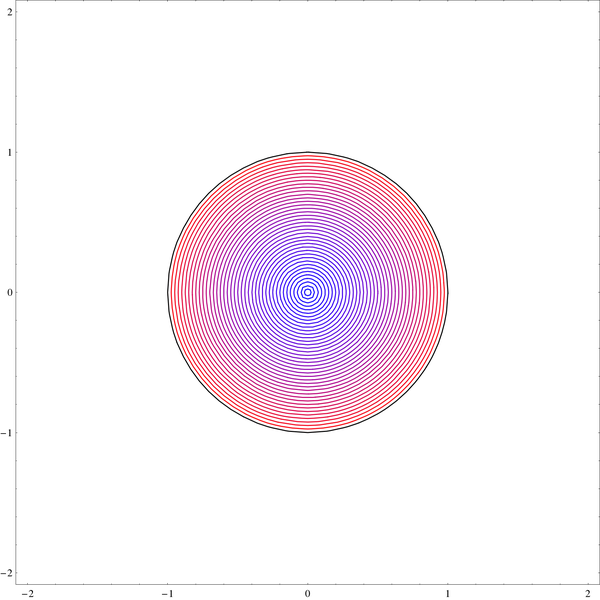
\includegraphics[width=\linewidth]{images/ball}
  \caption{The closed unit ball $D^2$ and a number of contours in $B^2\subset D^2$.}
  \label{ball}
\end{minipage}\hfill
\begin{minipage}{.45\textwidth}
  \centering
  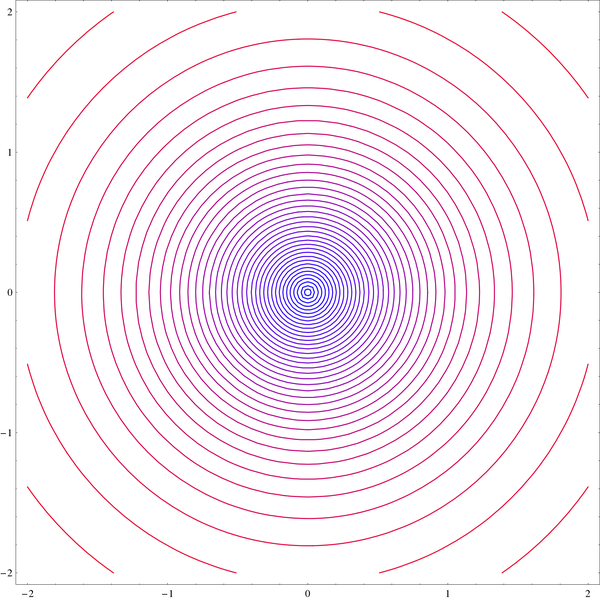
\includegraphics[width=\linewidth]{images/plane}
  \caption{The result of applying $\phi : B^2 \to \bbR^2$.}
  \label{plane}
\end{minipage}
\\
\begin{minipage}{.5\textwidth}
  \centering
  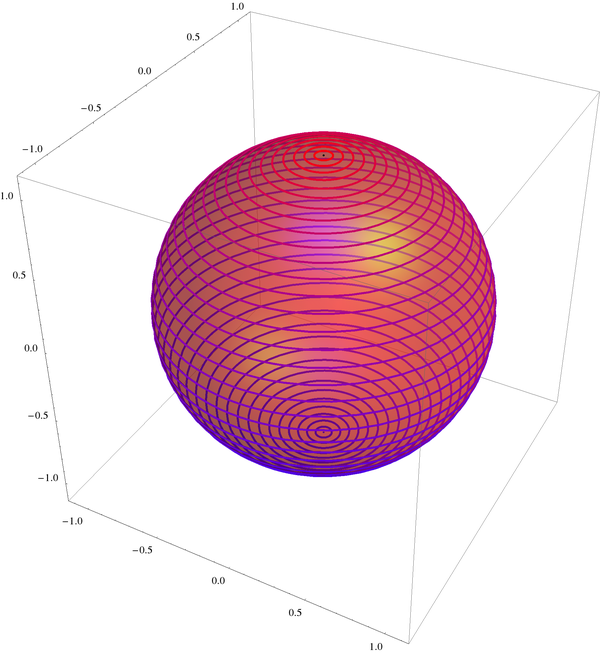
\includegraphics[width=\linewidth]{images/sphere}
  \caption{The contours in $S^2$ obtained by the map $g \circ \phi$.}
  \label{sphere}
\end{minipage}
\end{figure}

\subsection{Local compactness and one-point compactification}
